\documentclass[tikz,border=2pt]{standalone}
\usepackage{amsmath}
\usetikzlibrary{arrows.meta}
\begin{document}
% Remaining service time S_r(t) on [0,8]: services of length 1 (start 1) and 3 (start 3),
% triangles of area 1/2 and 9/2; time average 5/8 (green dashed).
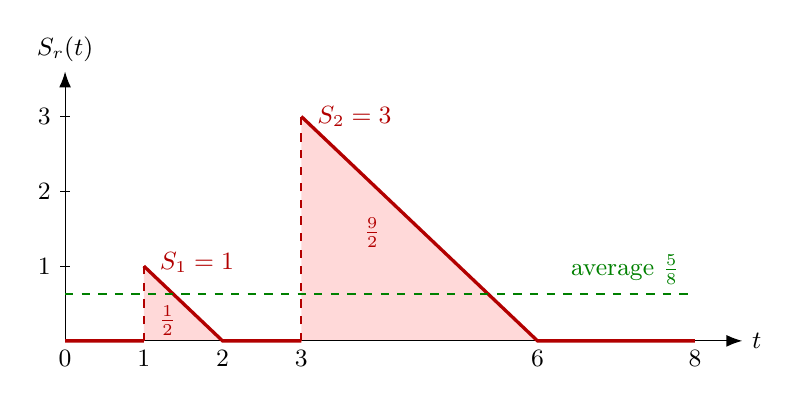
\begin{tikzpicture}[font=\small, >={Latex[length=2mm]}, x=1.0cm, y=0.95cm]
  \fill[red!15] (1,0) -- (1,1) -- (2,0) -- cycle;
  \fill[red!15] (3,0) -- (3,3) -- (6,0) -- cycle;
  \draw[->] (0,0) -- (8.6,0) node[right] {$t$};
  \draw[->] (0,0) -- (0,3.6) node[above] {$S_r(t)$};
  \foreach \y in {1,2,3} \draw (-0.06,\y) -- (0.06,\y) node[pos=0, left] {$\y$};
  \foreach \x in {1,2,3,6,8} \node[below] at (\x,0) {$\x$};
  \node[below] at (0,0) {$0$};
  \draw[red!70!black, very thick] (0,0) -- (1,0) (1,1) -- (2,0) -- (3,0) (3,3) -- (6,0) -- (8,0);
  \draw[red!70!black, thick, dashed] (1,0) -- (1,1) (3,0) -- (3,3);
  \node[red!70!black] at (1.3,0.27) {$\tfrac{1}{2}$};
  \node[red!70!black] at (3.9,1.45) {$\tfrac{9}{2}$};
  \node[red!70!black, anchor=west] at (3.08,3.0) {$S_2=3$};
  \node[red!70!black, anchor=west] at (1.08,1.05) {$S_1=1$};
  \draw[green!50!black, thick, dashed] (0,0.625) -- (8,0.625);
  \node[green!50!black, anchor=south west] at (6.3,0.625) {average $\tfrac{5}{8}$};
\end{tikzpicture}
\end{document}
